% Created 2021-02-01 Mon 11:06
% Intended LaTeX compiler: pdflatex
\documentclass{article}
\usepackage[utf8]{inputenc}
\usepackage[T1]{fontenc}
\usepackage{graphicx}
\usepackage{grffile}
\usepackage{longtable}
\usepackage{wrapfig}
\usepackage{rotating}
\usepackage[normalem]{ulem}
\usepackage{amsmath}
\usepackage{textcomp}
\usepackage{amssymb}
\usepackage{capt-of}
\usepackage{hyperref}
\usepackage{tikz}
\usetikzlibrary{shapes,arrows,calc,positioning}
\author{Sam Barrett}
\date{\today}
\title{Lecture 1}

\begin{document}

\maketitle

\section{Topic Overview}
\label{sec:org67939df}

Robot vision is a subset of Computer vision

\section{Introduction to Computer Vision}
\label{sec:orgdd022ac}

\subsection{A brief history of biological vision}
\label{sec:org9d27a8e}

\begin{itemize}
\item Vision can be traced back around 543M years.
\item Around this time, the number of different species \emph{exploaded}
\item We believe vision was responsible for this phase of evolution.
\item Humans have around 50\% of our neural tissue linked directly or indirectly to
\end{itemize}

\subsection{History of Computational Vision}
\label{sec:orgab35275}
One of the first academic works in computer vision was \emph{Block World} in 1963 by Larry Roberts. Here the world is translated into simple geometric shapes with the goal being to identify and understand what these shapes are.

Another influential figure in modern computer vision is David Marr.
\subsubsection{Though process of David Marr}
\label{sec:org4a1ae90}

Marr's process of thinking about computation representations of images follows very closely to what neuroscientists believe happens inside the human brain.

\begin{center}
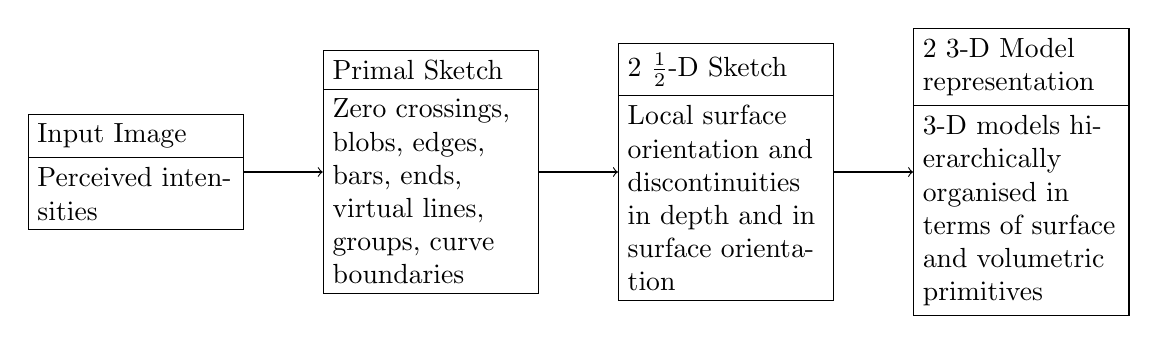
\begin{tikzpicture}[block/.style={
draw, rectangle split, rectangle split, rectangle split parts=2, rectangle split draw splits=true, text width = 25mm
}]
    \node [block] (b1) {
    Input Image
    \nodepart{two} Perceived intensities
  };

    \node [block, right=10mm of b1] (b2) {
    Primal Sketch
    \nodepart{two} Zero crossings, blobs, edges, bars, ends, virtual lines, groups, curve boundaries};

    \node [block, right=10mm of b2] (b3) {
    2 $\frac{1}{2}$-D Sketch
    \nodepart{two} Local surface orientation and discontinuities in depth and in surface orientation};

    \node [block, right=10mm of b3] (b4) {
    2 3-D Model representation
    \nodepart{two} 3-D models hierarchically organised in terms of surface and volumetric primitives};


  \draw[->] (b1) -- (b2);
  \draw[->] (b2) -- (b3);
  \draw[->] (b3) -- (b4);
\end{tikzpicture}
\end{center}

This interpretation is useful to understand the process of decomposing a image into computer-operable data.

Computer Vision is a multi-disciplinary field utilising expertise from Physics, Biology, Engineering, Computer Science and Psychology.

\subsection{Robot/ Computer Vision}

The main goal of computer vision is to automatically understand images and videos. It attempts to do this by computing properties of the 3D world from visual data. This is the \textit{measurement} phase.

To do this we require algorithms and representations to allow a machine to recognise objects, people, scenes and activities. This is known as \textit{perception} and \textit{interpretation} .

The next level is to implement algorithms to mine, search and interact with visual data. This is the \textit{search} and \textit{organisation} stage.

\subsubsection{Difficulty}

Human vision is not the goal, it is also flawed and can be fooled with optical illusions. Ideally, out computer systems would be immune to such issues.

What humans and computers ``\textit{see} '' differ greatly. Human vision produces a set of electrical impulses which our brain formats into what we know as an image. Computers interpret electrical signals differently, instead \textit{seeing} images as matrices of numbers.

There is also the issue of ambiguity arising from 3D scenes captured in 2 dimensions. Such as perspective changes.


Humans often use prior knowledge when interpreting an image. This is often useful but can lead to inaccuracies.

\section{Modern computer vision applications}

\subsection{Optical Character Recognition}

This system is widely used for scanning writing into a format that computers can work with. This is used for cheque processing, number plate recognition and handwriting recognition.

\subsection{Facial Recognition}

Another modern application of computer vision is facial authentication. This method for authorisation has been widely adopted and continues to see advancements to allow for things such as glasses, facial hair or different light levels.


\textbf{The rest of this lecture is just interesting applications \& videos, rewatch it if you are interested}

\subsection{Summary}

\begin{itemize}
  \item Robot/ computer vision is useful, interesting but difficult
  \item It is a growing and exciting field
  \item There are many \textit{cool} and important applications
\end{itemize}

\section{Module overview}


\end{document}
